\documentclass{article}

\usepackage[a4paper, total={6in, 9in}]{geometry} % Page margins
\usepackage[utf8]{inputenc}
\usepackage{amsmath, amssymb, mathtools, amsfonts, amsthm}
\usepackage{wasysym} % Smiley QED
\usepackage{eulervm} % Font
\usepackage{fancyhdr} % Custom headers and footers
\fancyhead[C]{\thepage} % Page numbering for center header
\usepackage{mdframed}
\usepackage{xcolor}
% list environments               
\usepackage{enumerate}            
\usepackage[shortlabels]{enumitem}      

% Code block environment
\usepackage{listings}            
\lstset{basicstyle = \ttfamily, mathescape}



% figure support
\usepackage{tikz}
\usepackage{graphicx}
\usepackage{subcaption} 
\usepackage{import}
\usepackage{xifthen}
\pdfminorversion=7
\usepackage{pdfpages}
\usepackage{transparent}

\pdfsuppresswarningpagegroup=1
\title{DSA: Exercise 3}
\author{David Sermoneta}
\begin{document}
\maketitle
\section*{Exercise 1:}
\subsection*{Exercise 1.a)}
\begin{lstlisting}[numbers = left]
  : 5 9
  : 5
  : 9
  : LR 5 9
  : 3 8 2
  : 3
  : 8 2
  : 8
  : 2
  : LR 8 2
  : LR 3 8
  : LR 9 8 
\end{lstlisting}

\subsection*{Exercise 1.b)}
Since we call the function twice, that sets $a = 2$, and each call halves $n$ by 2,
this gives us $b=2$. Further, we have $3$ \texttt{PRINT} statements, as well
as 2 operations that take constant time, thus $d = 0$. We get the following form: \[
T(n) = 2T\left(\left\lfloor \frac{n}{2} \right\rfloor \right) + 5\Theta(1) .
\] Since $2 > 2^{0}$, we have that  \[
T(n) = \Theta(n^{\log_b(a)}) = \Theta(n),
\] and we are done.


\subsection*{Exercise 1.c)}
Apart from the obvious: getting rid of the print statements, there isn't anything
else to do. We can explain this via the following reasoning. apart from the 
print statements, there are: 
\begin{enumerate}
    \item Base case of the recursion formula,
    \item initializing of the variable $k$ that is used in the rest of the code,
    \item calling the function on the sliced list \texttt{A[1 : k} and  \texttt{
        A[k : A.length]}.
\end{enumerate}
Removing any of these, would result either in the function not 
ending, a code error, or a function that 
does not find the maximum of a list, but rather, a shorter version of the list.
So the answer is, one can only remove the three print stamements to have the
algorithm still find the maximum element of a given array.

\section*{Exercise 2:}

\begin{figure}[htpb]
    \centering
 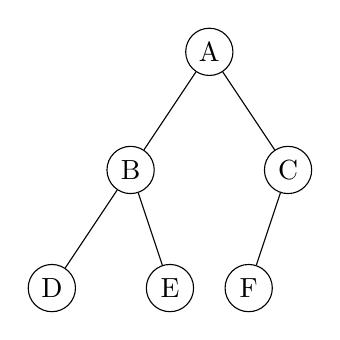
\begin{tikzpicture}[every node/.style={circle, draw, inner sep=2pt, minimum size=6mm}]
     \node (A) at (0,0) {A};
     \node (B) at (-1,-1.5) {B};
     \node (C) at (1,-1.5) {C};
     \node (D) at (-2,-3) {D};
     \node (E) at (-0.5,-3) {E};
     \node (F) at (0.5,-3) {F};
      
     \draw (A) -- (B);
     \draw (A) -- (C);
     \draw (B) -- (D);
     \draw (B) -- (E);
     \draw (C) -- (F);
 \end{tikzpicture}
 \caption{Graph with both inorder and preorder traversal}
\end{figure}
\begin{figure}[htpb]
    \centering
\begin{tikzpicture}[every node/.style={circle, draw, inner sep=2pt, minimum size=6mm}]     
   \node (A) at (0,0) {A};
    \node (B) at (-1,-1.5) {B};
    \node (C) at (-4,-6) {C};
    \node (D) at (-2,-3) {D};
    \node (E) at (-3,-4.5) {E};
    \node (F) at (-5,-7.5) {F};
                 
    \draw (A) -- (B);
    \draw (B) -- (D);
    \draw (D) -- (E);                                                                                                    
    \draw (E) -- (C);
    \draw (C) -- (F);
\end{tikzpicture}
\caption{Graph with only preorder traversal specified, it is not the same as
the one in figure 1, so the preorder traversal does not determine $T$ uniquely.}
\end{figure}
\section*{Exercise 3:}
For graph ($i$), we have height($T_{i}$) = $3$, depth($3$) = $2$, and it neither
FB, NC nor C. \\
For graph ($ii$), we have height($T_{ii}$) = $3$, depth($3$) = $1$, and it is all of
the above.  \\
For graph ($iii$), we have height($T_{iii}$) = $2$, depth($3$) = $2$, and it is
only NC.  \\
For graph ($iv$), we have height($T_{iv}$) = $2$, depth($3$) = $0$, and it is only
FB. 
\section*{Exercise 4:}
\begin{lstlisting}[numbers = left]      
MERGESORT(A,1,3) 
MERGESORT(A,1,2) 
MERGESORT(A,1,1) 
MERGESORT(A,2,2) 
MERGE(A,1,1,2) $\to$ [2,6]
MERGESORT(A,3,3)
MERGE(A,1,2,3) $\to$ [2,3,6]
\end{lstlisting}

\section*{Exercise 5:}
\subsection*{Solution to 5.a}

\begin{figure}[htpb]
    \centering
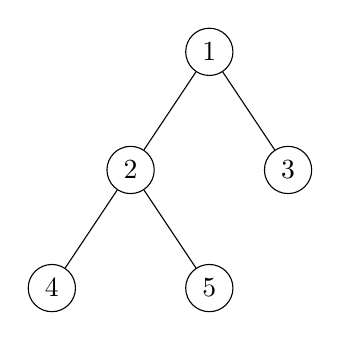
\begin{tikzpicture}[every node/.style={circle, draw, inner sep=2pt, minimum size=6mm}] 
    \node (A) at (0,0) {1};
    \node (B) at (-1,-1.5) {2};
    \node (C) at (1, -1.5) {3};
    \node (D) at (-2, -3) {4};
    \node (E) at (0, -3) {5};

    \draw (A) -- (B);
    \draw (A) -- (C);
    \draw (B) -- (D);
    \draw (B) -- (E);
\end{tikzpicture}
\caption{Array $A$ as a binary heap tree.}
\end{figure}
\newpage
\subsection*{Solution to 5.b}
The first time upon calling \texttt{Build\_Max\_Heap($A$)}, we get
that the indices that violate the max-heap property are $2$ and $3$, since the parent 
of $2$ and $3$ is smaller than both respectively. That is, $A$\texttt{[parent(2)]}$<A$
\texttt{[2]} and same for $3$. 
Calling on \texttt{Build\_Max\_Heap($A$)} forces us to call on \texttt{Max\_Heapify($A$,
2}, and later, \texttt{Max\_heapify($A$,1)},
which gives us the following graphs representations of the subtrees rooted at the
index we are calling (specified in the figures below):
\begin{figure}[htpb]
    \centering
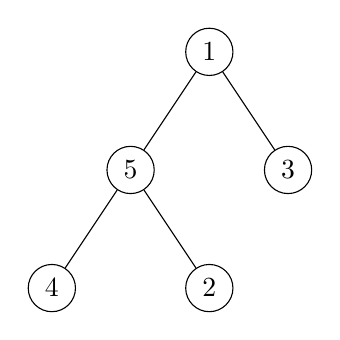
\begin{tikzpicture}[every node/.style={circle, draw, inner sep=2pt, minimum size=6mm}] 
    \node (A) at (0,0) {1};
    \node (B) at (-1,-1.5) {5};
    \node (C) at (1, -1.5) {3};
    \node (D) at (-2, -3) {4};
    \node (E) at (0, -3) {2};

    \draw (A) -- (B);
    \draw (A) -- (C);
    \draw (B) -- (D);
    \draw (B) -- (E);
\end{tikzpicture}
\caption{Array $A$ as a binary heap tree after \texttt{Max\_Heapify($A$,2).}}
\end{figure}
The calling of \texttt{Max\_Heapify($A$,1)} gives us another call, namely on index 
$2$, which will be the element $1$:
\begin{figure}[htpb]
    \begin{subfigure}[h]{0.4\linewidth}
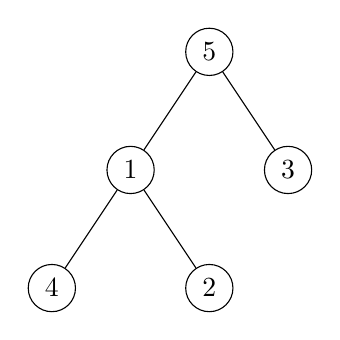
\begin{tikzpicture}[every node/.style={circle, draw, inner sep=2pt, minimum size=6mm}] 
    \node (A) at (0,0) {5};
    \node (B) at (-1,-1.5) {1};
    \node (C) at (1, -1.5) {3};
    \node (D) at (-2, -3) {4};
    \node (E) at (0, -3) {2};

    \draw (A) -- (B);
    \draw (A) -- (C);
    \draw (B) -- (D);
    \draw (B) -- (E);
\end{tikzpicture}
\caption{Binary heap representation after call of \texttt{Max\_Heapify($A$,2)}.
Now the index $4$ and $5$ violate the Max heap property, that is, the elements $4$ and
$2$.}
\end{subfigure} 
\hfill
\begin{subfigure}[h]{0.4\linewidth}
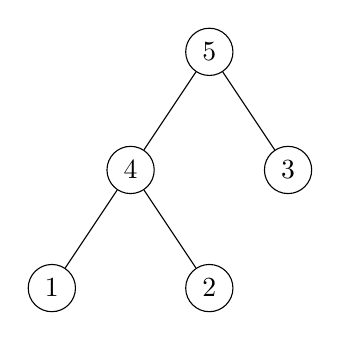
\begin{tikzpicture}[every node/.style={circle, draw, inner sep=2pt, minimum size=6mm}] 
    \node (A) at (0,0) {5};
    \node (B) at (-1,-1.5) {4};
    \node (C) at (1, -1.5) {3};
    \node (D) at (-2, -3) {1};
    \node (E) at (0, -3) {2};

    \draw (A) -- (B);
    \draw (A) -- (C);
    \draw (B) -- (D);
    \draw (B) -- (E);
\end{tikzpicture}
\caption{Binary heap representation after call of \texttt{Max\_Heapify($A$,2)}. 
Now there are no nodes that violate the Max Heap property and thus we are done.}
\end{subfigure}
\end{figure}
\newpage

\subsection*{Solution to 5.c}



\begin{figure}[htpb]
    \begin{subfigure}[h]{0.4\linewidth}
    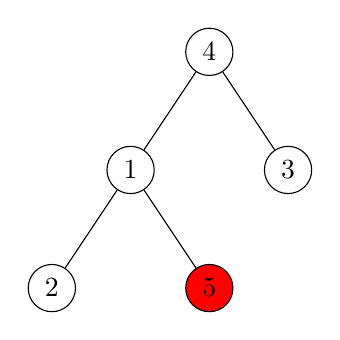
\begin{tikzpicture}[every node/.style={circle, draw, inner sep=2pt, minimum size=6mm}] 
    \node (A) at (0,0) {4};
    \node (B) at (-1,-1.5) {1};
    \node (C) at (1, -1.5) {3};
    \node (D) at (-2, -3) {2};
    \node[fill=red] (E) at (0, -3) {5};

    \draw (A) -- (B);
    \draw (A) -- (C);
    \draw (B) -- (D);
    \draw (B) -- (E);
\end{tikzpicture}
\caption{\texttt{i = 5}}
\end{subfigure}
\hfill
    \begin{subfigure}[h]{0.4\linewidth}
    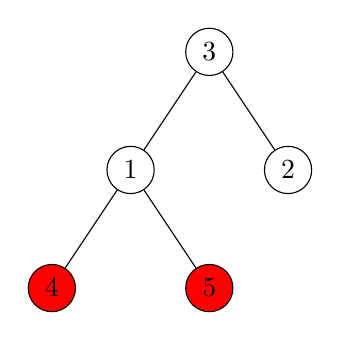
\begin{tikzpicture}[every node/.style={circle, draw, inner sep=2pt, minimum size=6mm}] 
    \node (A) at (0,0) {3};
    \node (B) at (-1,-1.5) {1};
    \node (C) at (1, -1.5) {2};
    \node[fill = red] (D) at (-2, -3) {4};
    \node[fill=red] (E) at (0, -3) {5};
    
    \draw (A) -- (B);
    \draw (A) -- (C);
    \draw (B) -- (D);
    \draw (B) -- (E);
\end{tikzpicture}
\caption{\texttt{i = 4}}
\end{subfigure}
\hfill 
\begin{subfigure}[h]{0.4\linewidth}
    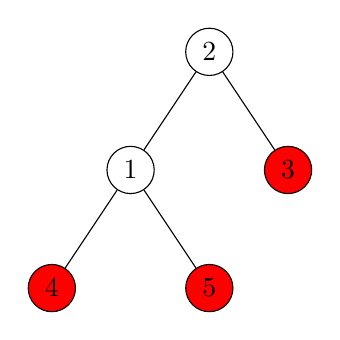
\begin{tikzpicture}[every node/.style={circle, draw, inner sep=2pt, minimum size=6mm}] 
    \node (A) at (0,0) {2};
    \node (B) at (-1,-1.5) {1};
    \node[fill = red] (C) at (1, -1.5) {3};
    \node[fill = red] (D) at (-2, -3) {4};
    \node[fill=red] (E) at (0, -3) {5};
    
    \draw (A) -- (B);
    \draw (A) -- (C);
    \draw (B) -- (D);
    \draw (B) -- (E);
\end{tikzpicture}
\caption{\texttt{i = 3}}
\end{subfigure}
\hfill
\hfill
\begin{subfigure}[h]{0.4\linewidth}
    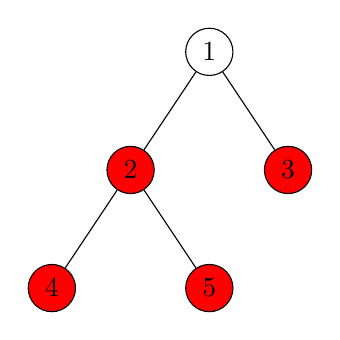
\begin{tikzpicture}[every node/.style={circle, draw, inner sep=2pt, minimum size=6mm}] 
    \node (A) at (0,0) {1};
    \node[fill = red] (B) at (-1,-1.5) {2};
    \node[fill = red] (C) at (1, -1.5) {3};
    \node[fill = red] (D) at (-2, -3) {4};
    \node[fill=red] (E) at (0, -3) {5};
    
    \draw (A) -- (B);
    \draw (A) -- (C);
    \draw (B) -- (D);
    \draw (B) -- (E);
\end{tikzpicture}
\caption{\texttt{i = 2}}
\end{subfigure}
\end{figure}

\section*{Exercise 6:}
Let \texttt{A}$ = \{a_1,a_2,\ldots,a_{n}\} $ be the set of coins. If we chose to 
weigh half of the coins from $a_1,\ldots,a_{k}$, where $k= \left\lfloor 
\frac{n}{2}\right\rfloor$, we'd expect it to weigh  $k\cdot w$ if our
CF coin wasn't there, and so we'll know in which half of the set it is by
seeing if the weight deviates from it. Repeating this process should 
yield us our counterfeit (CF) coin after a finite number of iterations.
In pseudocode, this becomes
\begin{lstlisting}[numbers = left]
def SCF(A, left, right)
    IF left == right: return left
    middle = left  + right // 2
    expected_value = (middle - left + 1)*$w$
    weight = Weigh(A[left : middle]) 
    IF expected_value != weight
        return SCF(A, left, middle)
    ELSE: return SCF(A, middle+1, right)
\end{lstlisting}
Here \texttt{Weigh(A[left : middle]} just returns the weight of the
elements left to (including) middle of \texttt{A}. \\
When we first call the algorithm, we have that the CF coin is either
in (1.) \texttt{A[left:middle]}, or in (2.) \texttt{A[middle+1:right]}.
So our loop invariant is just to show that for each recursion, the CF 
with index $i$ is always between  \texttt{left} and \texttt{middle} if 
the last  \texttt{IF}  statement is satisfied, or between 
\texttt{middle+1} and  \texttt{right} otherwise.
The \texttt{IF} statement is only satisfied when the weight of 
\texttt{A[left:middle]} deviates from the expected value, meaning the
CF coin is in there. So calling  \texttt{SCF} with  \texttt{right=middle}
gives us that the loop invariant is satisfied.
\newpage 
\noindent If not, then that means that \texttt{expected\_value == weight}, and so 
$i$ must be in the second half of \texttt{A}, which means that in the 
next recursion, the  CF coin will be between \texttt{middle+1} and
\texttt{right}, and so when we call  \texttt{SCF} with  
\texttt{left==middle+1}, we get that the loop invariant is also
satisfied. \\
To find out the amount of weighings this algorithm has, suppose 
$|$\texttt{A}$|=n$, and that $d$ is the amount of weighings we did before 
finding the CF coin. Then since we divide \texttt{A} in two after each 
weighing, that must mean that we have divided $n$ by $2^{d}$ times. 
meaning that $\frac{n}{2^{d}}=1$ since that is when the algorithms 
terminates, and we get afters ome manipulation that $d= \log_2(n)$.
So the amount of weighings made is $\log_2(n)$ for an array of size $n$.
\end{document}
